<<<<<<< HEAD
%%%%%%%%%%%%%%%%%%%%%%%%%%%%%%%%%%%%%%%%%%%
%%%%%%  STYLE 17
%%%%%%%%%%%%%%%%%%%%%%%%%%%%%%%%%%%%%%%%%%%
\newgeometry{left=7cm,right=2cm, marginparsep=15pt, marginparwidth=4.2cm,top=2cm,%
reversemarginpar}
\cxset{style17/.style={
 name={},
 numbering=arabic,
 number font-size=\huge,
 number font-family=\sffamily,
 number font-weight=\bfseries,
 number before=,
 number dot=.,
 number color=\color{purple},
 number after=\thinspace,
 number position=rightname,
 chapter font-family=\sffamily,
 chapter font-weight=\bfseries,
 chapter font-size=\LARGE,
 chapter before={\vspace*{20pt}\par\hfill},
 chapter after={},
 chapter color={black!90},
 title beforeskip={},
 title afterskip={\vspace*{70pt}\par},
 title before={},
 title after={},
 title font-family=\sffamily,
 title font-color=\color{purple},
 title font-shape=\upshape,
 title font-weight=\bfseries,
 title font-size=\huge,
 section numbering=none,
 section beforeskip=10pt,
 section afterskip=10pt,
 section font-family=\rmfamily,
 section font-shape=\slshape,
 geometry marginparwidth=4.5cm,
 geometry marginparsep=20pt}}
\cxset{style17}

\chapter{Introduction to Style Seventeen}

I tend to favour this design for books that have a lot of pictures. It brings the design into the margins and leaves plentiful white space in the margins. From a programming point of view the chapter is the opposite of openany. It has to open on an odd number.

\marginpar{%
\vspace*{0.2\textheight}
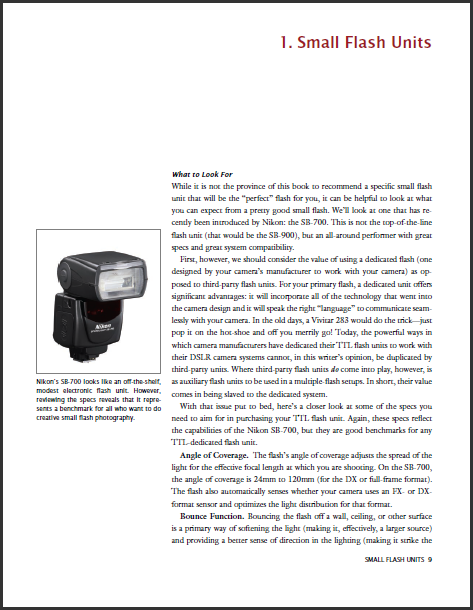
\includegraphics[width=\marginparwidth]{./chapters/chapter17}\par
{\footnotesize\lorem}
}

\section{Use the margins}

Adjustments to the geometry layout can be carried out temporarily or permanently via the use of keys and
the geometry package. These are probably the less problematic and easier to set geometry settings.

\section{Margin notes}

Marginal notes use the same mechanism as
floats to communicate with the \cs{output} routine. Marginal notes are distinguished from
floats by having a negative placement specification. The command
\cs{marginpar}\oarg{left text}\marg{right text} generates a marginal note in a parbox,
using LTEXT if it's on the left and RTEXT if it's on the right.
(Default is RTEXT = LTEXT.) It uses the following parameters.
\cs{marginparwidth}: Width of marginal notes.
\cs{marginparsep}: Distance between marginal note and text.
the page layout to determine how to move the marginal
note into the margin. E.g.,

\begin{tcolorbox}
\begin{lstlisting}
\@leftmarginskip ==\hskip -\marginparwidth \hskip -\marginparsep .
\end{lstlisting}
\end{tcolorbox}

\cs{marginparpush} Minimum vertical separation between \cs{marginpar}'s
Marginal notes are normally put on the outside of the page
if @mparswitch = true, and on the right if @mparswitch = false.
The command \cs{reversemarginpar} reverses the side where they
are put. \cs{normalmarginpar} undoes \cs{reversemarginpar}.
These commands have no effect for two-column output.
\marginpar{\footnotesize \textsc{\bfseries NOTE:} if two marginal notes appear on the same line of
text, then the second one could appear on the next page, in
a funny position.}
\section{Sample text}
\lipsum[2-4]

\restoregeometry
=======
%%%%%%%%%%%%%%%%%%%%%%%%%%%%%%%%%%%%%%%%%%%
%%%%%%  STYLE 17
%%%%%%%%%%%%%%%%%%%%%%%%%%%%%%%%%%%%%%%%%%%
\newgeometry{left=7cm,right=2cm, marginparsep=15pt, marginparwidth=4.2cm,top=2cm,%
reversemarginpar}
\cxset{style17/.style={
 name={},
 numbering=arabic,
 number font-size=\huge,
 number font-family=\sffamily,
 number font-weight=\bfseries,
 number before=,
 number dot=.,
 number color=\color{purple},
 number after=\thinspace,
 number position=rightname,
 chapter font-family=\sffamily,
 chapter font-weight=\bfseries,
 chapter font-size=\LARGE,
 chapter before={\vspace*{20pt}\par\hfill},
 chapter after={},
 chapter color={black!90},
 title beforeskip={},
 title afterskip={\vspace*{70pt}\par},
 title before={},
 title after={},
 title font-family=\sffamily,
 title font-color=\color{purple},
 title font-shape=\upshape,
 title font-weight=\bfseries,
 title font-size=\huge,
 section numbering=none,
 section beforeskip=10pt,
 section afterskip=10pt,
 section font-family=\rmfamily,
 section font-shape=\slshape,
 geometry marginparwidth=4.5cm,
 geometry marginparsep=20pt}}
\cxset{style17}

\chapter{Introduction to Style Seventeen}

I tend to favour this design for books that have a lot of pictures. It brings the design into the margins and leaves plentiful white space in the margins. From a programming point of view the chapter is the opposite of openany. It has to open on an odd number.

\marginpar{%
\vspace*{0.2\textheight}
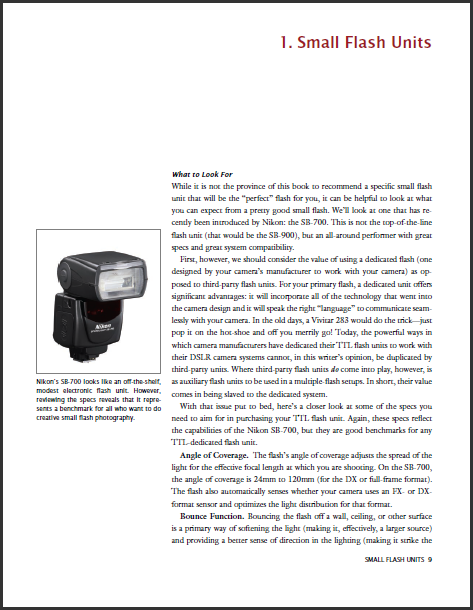
\includegraphics[width=\marginparwidth]{./chapters/chapter17}\par
{\footnotesize\lorem}
}

\section{Use the margins}

Adjustments to the geometry layout can be carried out temporarily or permanently via the use of keys and
the geometry package. These are probably the less problematic and easier to set geometry settings.

\section{Margin notes}

Marginal notes use the same mechanism as
floats to communicate with the \cs{output} routine. Marginal notes are distinguished from
floats by having a negative placement specification. The command
\cs{marginpar}\oarg{left text}\marg{right text} generates a marginal note in a parbox,
using LTEXT if it's on the left and RTEXT if it's on the right.
(Default is RTEXT = LTEXT.) It uses the following parameters.
\cs{marginparwidth}: Width of marginal notes.
\cs{marginparsep}: Distance between marginal note and text.
the page layout to determine how to move the marginal
note into the margin. E.g.,

\begin{tcolorbox}
\begin{lstlisting}
\@leftmarginskip ==\hskip -\marginparwidth \hskip -\marginparsep .
\end{lstlisting}
\end{tcolorbox}

\cs{marginparpush} Minimum vertical separation between \cs{marginpar}'s
Marginal notes are normally put on the outside of the page
if @mparswitch = true, and on the right if @mparswitch = false.
The command \cs{reversemarginpar} reverses the side where they
are put. \cs{normalmarginpar} undoes \cs{reversemarginpar}.
These commands have no effect for two-column output.
\marginpar{\footnotesize \textsc{\bfseries NOTE:} if two marginal notes appear on the same line of
text, then the second one could appear on the next page, in
a funny position.}
\section{Sample text}
\lipsum[2-4]

\restoregeometry
>>>>>>> merged
